% Options for packages loaded elsewhere
\PassOptionsToPackage{unicode}{hyperref}
\PassOptionsToPackage{hyphens}{url}
%
\documentclass[
]{article}

\usepackage{lmodern}
\usepackage{amssymb,amsmath}
\usepackage{ifxetex,ifluatex}
\ifnum 0\ifxetex 1\fi\ifluatex 1\fi=0 % if pdftex
  \usepackage[T1]{fontenc}
  \usepackage[utf8]{inputenc}
  \usepackage{textcomp} % provide euro and other symbols
\else % if luatex or xetex
  \usepackage{unicode-math}
  \defaultfontfeatures{Scale=MatchLowercase}
  \defaultfontfeatures[\rmfamily]{Ligatures=TeX,Scale=1}
\fi
% Use upquote if available, for straight quotes in verbatim environments
\IfFileExists{upquote.sty}{\usepackage{upquote}}{}
\IfFileExists{microtype.sty}{% use microtype if available
  \usepackage[]{microtype}
  \UseMicrotypeSet[protrusion]{basicmath} % disable protrusion for tt fonts
}{}
\makeatletter
\@ifundefined{KOMAClassName}{% if non-KOMA class
  \IfFileExists{parskip.sty}{%
    \usepackage{parskip}
  }{% else
    \setlength{\parindent}{0pt}
    \setlength{\parskip}{6pt plus 2pt minus 1pt}}
}{% if KOMA class
  \KOMAoptions{parskip=half}}
\makeatother
\usepackage{xcolor}
\IfFileExists{xurl.sty}{\usepackage{xurl}}{} % add URL line breaks if available
\IfFileExists{bookmark.sty}{\usepackage{bookmark}}{\usepackage{hyperref}}
\hypersetup{
  pdftitle={Photomoss workflow},
  pdfauthor={Manuel Molina},
  hidelinks,
  pdfcreator={LaTeX via pandoc}}
\urlstyle{same} % disable monospaced font for URLs
\usepackage{graphicx}
\makeatletter
\def\maxwidth{\ifdim\Gin@nat@width>\linewidth\linewidth\else\Gin@nat@width\fi}
\def\maxheight{\ifdim\Gin@nat@height>\textheight\textheight\else\Gin@nat@height\fi}
\makeatother
% Scale images if necessary, so that they will not overflow the page
% margins by default, and it is still possible to overwrite the defaults
% using explicit options in \includegraphics[width, height, ...]{}
\setkeys{Gin}{width=\maxwidth,height=\maxheight,keepaspectratio}
% Set default figure placement to htbp
\makeatletter
\def\fps@figure{htbp}
\makeatother
\setlength{\emergencystretch}{3em} % prevent overfull lines
\providecommand{\tightlist}{%
  \setlength{\itemsep}{0pt}\setlength{\parskip}{0pt}}
\setcounter{secnumdepth}{-\maxdimen} % remove section numbering
\ifluatex
  \usepackage{selnolig}  % disable illegal ligatures
\fi

\title{Photomoss workflow}
\author{Manuel Molina}
\date{24/7/2020}

\begin{document}
\maketitle

\hypertarget{what-is-photomoss}{%
\subsection{\texorpdfstring{What is
\emph{photomoss}?}{What is photomoss?}}\label{what-is-photomoss}}

\emph{\textbf{Photomoss}} is a developement from
\textbf{mosscoder/crustcover} package
(https://github.com/mosscoder/crustCover). As with \emph{crustcover},
with \emph{\textbf{photomoss}} we will meassure the size of moss
occupied areas in field or lab experiments. As \emph{crustcover} achieve this duty, we use the same principles as (Fischer2012)that 
take advantage of Near InfraRed (NIR) and RGB images.
With the color channels of this images, we can achieve several spectral
indexes that will allow to measure moss surface or physiological
condition. In contrast with \emph{crustcover} that measures seven index,
\emph{photomoss} can use a great set of 19 spectral indexes. As
\emph{crust cover}, \emph{photomoss} core function can calculate moss
area using a given spectral index and implementigg a custom threshold
value, but in addition, it can apply an authomatic segmentation
following a set of 12 different segmentation methods if needed. Other
additional functionalities of \emph{photomoss} in comparison with
\emph{crustcover} are the semiautomatisation of annalysis area over the
image, and a segmentation accuracy test functionality, to test the
segmentation accuracy comparing the calculated surfaces with a the true
moss area from a binary mask image done with ImageJ.

\hypertarget{installing-photomoss}{%
\subsection{Installing photomoss}\label{installing-photomoss}}

we need to install \emph{devtools} package:

\begin{verbatim}
if(require(devtools)!=T){
  install.packages('devtools')
  require(devtools)
}
\end{verbatim}

Then we install \emph{photomoss} from my GitHub branch:

\begin{verbatim}
install_github("scolymushisp/photomoss")
library(photomoss)
\end{verbatim}

Maybe you need to install some other packages, so be aware of warnings
and install them.

\hypertarget{set-working-directory-structure}{%
\subsection{Set working directory
structure}\label{set-working-directory-structure}}

This is an important step, because the function searches the images in a
directory structure that has to be always the same.

Our working directory have to include the following folders and files:

\begin{itemize}
\tightlist
\item
  \emph{\textbf{vis}} folder: this folder includes the RGB images.
\item
  \emph{\textbf{nir}} folder: this folder includes the NIR images.
\item
  \emph{\textbf{mask}} folder: this folder includes the binary mask
  images. Mandatory if in the function \emph{ccspectral.df} the argument
  \emph{manual.mask.test = T}.
\end{itemize}

\begin{itemize}
\item
  \emph{\textbf{rois}} folder: this folder includes the \emph{regions of
  interest} (\emph{\textbf{rois}})for each pair of nir and vis images
  (or for each triad of nir, vis, mask if it is the case). A \emph{roi}
  is the region of the image where we can find the moss sample to
  analyze. It is necesary to previously create this files using
  \emph{ImageJ}.

  \begin{itemize}
  \tightlist
  \item
    \textbf{Attention.1}: if the nir and vis images contain several
    samples the \emph{\textbf{rois}} folder must include as many
    subfolders samples. In each subfolder we must put the .roi files for
    that nir-vis image. So, if an image includes four samples, as in
    Figure 1, and we want to analyze them all, we need to have four
    rois. in that subfolder.
  \item
    \textbf{Attention.2}: the .roi files in each subfolder must be
    ordered in the same way as the \emph{names.csv} file (we will talk
    about it later.)
  \end{itemize}
\end{itemize}

\hypertarget{set-working-directory}{%
\subsection{Set working directory}\label{set-working-directory}}

\begin{verbatim}
wd #your working directory
setwd (wd)
tif.path <- getwd()
\end{verbatim}

\hypertarget{start-with-the-functions}{%
\subsection{Start with the functions}\label{start-with-the-functions}}

\hypertarget{chart.from.tif}{%
\subsubsection{\texorpdfstring{\emph{chart.from.tif}}{chart.from.tif}}\label{chart.from.tif}}

We create the chart object (a list of polygons) with the
\emph{chart.from.tif} function. To do this we click over the color cells
chart in the image. Importantnote: folow the order as indicated in the
figure.

\begin{verbatim}
chart<- chart.from.tif(tif.path) 
\end{verbatim}

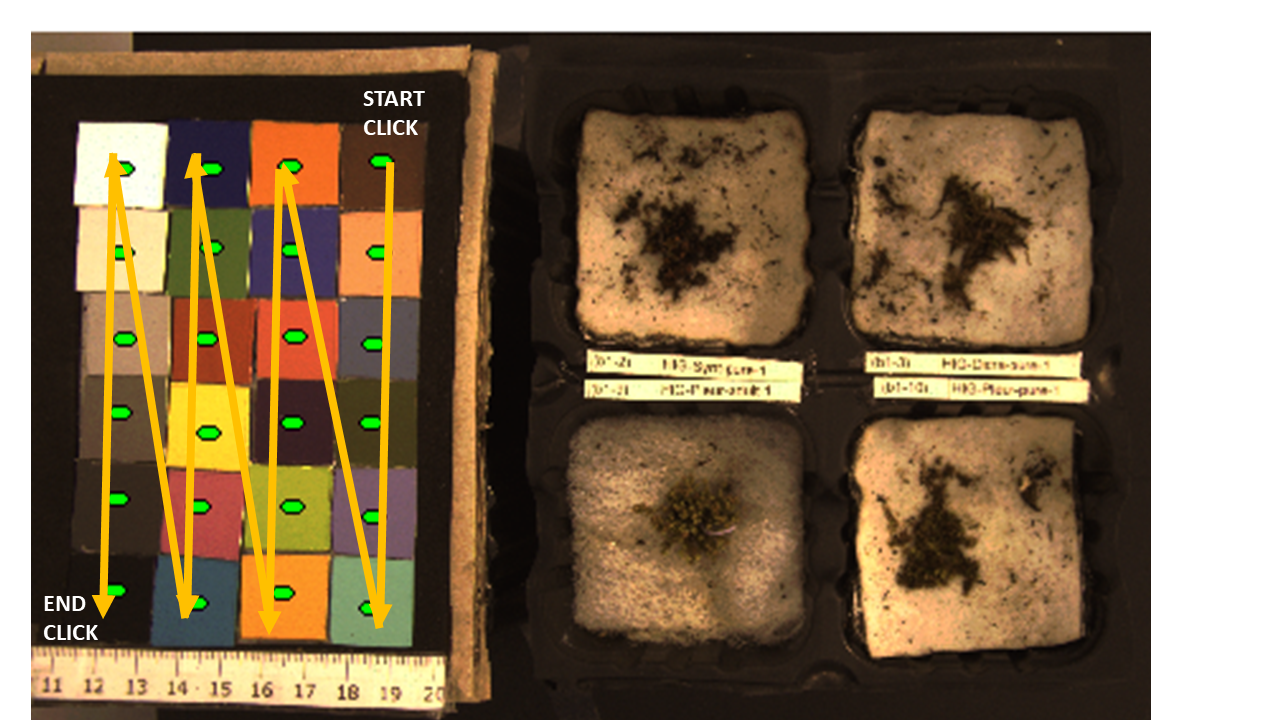
\includegraphics[width=5.83333in,height=3.28125in]{chart.png}

Figure 1

\hypertarget{roi2polygon.2-and-extractpix.from.poly.}{%
\subsection{\texorpdfstring{\emph{roi2polygon.2} and
\emph{extractPIX.from.Poly}.}{roi2polygon.2 and extractPIX.from.Poly.}}\label{roi2polygon.2-and-extractpix.from.poly.}}

Now we use the \emph{roi2polygon.2} function to create a readable
polygon files (\emph{polys} object) from the ImageJ .roi files. Then we
crop the pixels that fell inside the polygons and obtain a list og
ploygon data.frame (\emph{obs.areas} object)

\begin{verbatim}
roi.paths<- list.files(path = "./rois",pattern=".roi$",full.names = T, recursive = T)

polys <- lapply(roi.paths, roi2polygon.2, tif.path)
\end{verbatim}

\hypertarget{ccspectral.df}{%
\subsection{\texorpdfstring{\emph{ccspectral.df}}{ccspectral.df}}\label{ccspectral.df}}

This is the core function of photomoss.

The basic result of this function is a dataframe with the \textbf{areas
in number of pixels} of background and moss area for each sample. If
argument \emph{descrip = T} the descriptive statistics of the different
areas.

\hypertarget{arguments-in-ccspectral.df}{%
\section{\texorpdfstring{Arguments in
\emph{ccspectral.df}:}{Arguments in ccspectral.df:}}\label{arguments-in-ccspectral.df}}

\begin{itemize}
\tightlist
\item
  \textbf{tif.path}: the path of the working directory where are the
  \emph{\textbf{vis}}, \emph{\textbf{nir}}, \emph{\textbf{mask}},
  \emph{\textbf{rois}} folders and \emph{\textbf{names.csv}} file.
\item
  \textbf{chart}: polygon list obtained with \emph{chart.from.tif}
  function.
\item
  \textbf{obs.areas}: list of polygons data.frame obtained with
  \emph{extractPIX.from.Poly} function.
\item
  \textbf{pdf}: logical, to present the results in image and histogram
  of moss areas. Default = F.
\item
  \textbf{calculate.thresh}: logical, to Calculate autothreshold.
  Default = T.
\item
  \textbf{descrip}: logical, to calculate statistical descriptors of
  index value in the moss area, backround area,\ldots{} Default = F.
\item
  \textbf{manual.mask.test}: logical, if you want to test the accuracy
  of image segmentation comparing with handmade drawn moss area. Default
  = F,
\item
  \textbf{index.}: character with what index you want to calculate. By
  default, all options: \emph{index.} = c(``NDVI'', ``SR'', ``MSAVI'',
  ``EVI'', ``CI'', ``BSCI'', ``BI'',``NORR'', ``NORG'', ``NORB'',
  ``EXR'', ``EXG'',``EXB'', ``EXGR'', ``CIVE'', ``VEG'', ``HUE'',
  ``SAT'', ``VAL'')
  \bigskip
  \\
  The options represent the folowing indexes:
  \medskip 
   \begin{enumerate}
    	\item \emph{NDVI}: \textbf{Normalized Differential Vegetation Index.}
    	Is the normalize difference beween Near Infrared (NIR) values and visible RED values. 
    	NDVI is used in teledetection aplications to measure physiological active vegetation, 
    	because clorophyl absorbs Red and reflects NIR. NDVI scales between -1 and 1, being 1 
    	the value of an active green leaf.   
    	\[
    	NDVI = \frac{(NIR - RED)}{(NIR + RED)}  
    	\]
        \item \emph{SR} \textbf{Simple Ratio}. Te difference between NIR value and Red value, 
        without standarisation. It's an uscaled index
        \[
    	SR = NIR - RED
    	\] 
        \item \emph{MSAVI}:  \textbf{Second Modified Soil Adjusted Vegetation Index.} Use a 
        self-adjusting soil factor to reduce background soil influence. MSAVI scales between 
        -1 and 1 (Qi1994). 
        \[
        MSAVI = \frac{2\times NIR + 1 - \sqrt{(2 x NIR + 1)2 - 8 \times (NIR -RED)}}{2}
    	\]
        \item \emph{EVI}:  \textbf{Enhanced Vegetation Index.} Is an enhanced NDVI that 
        includes a soil adjustment factor and  uses the blue band to correct the  red  band  
        atmospheric aerosol distortion.(Liu1995), (Huete1999)        
          \[
          EVI = \frac{2.5 x ((NIR - RED) }{(NIR + 6 \times RED - 7.5 \times BLUE + 1))} 
          \]
        \item \emph{CI}: \textbf{Crust Index.} Is based on the standarized difference between  
        RED and BLUE bands. It's an index develloped to detect Biological Solil Crust with 
        cyaniobacteria. (KARNIELLI1997)
         \[
         CI = 1 - \frac{RED - BLUE}{RED + BLUE} 
         \]
        \item \emph{BSCI}: \textbf{Biological Soil Crust Index.} Is based on GREEN, RED and 
        NIR bands. This index was designed to exacerbate the spectral differences between 
        Biological Soil Crusts and bares sand, dry plants and green plants. Include an 
        adjustment factor with value 2 to magnify the absolute difference between RED and 
        GREEN bands (Chen2005)
         \[
         BSCI = \frac{(1 - 2 \times |RED - GREEN|)}{mean(GREEN, RED, NIR)}   
         \]
\item \emph{BI}: Brightness Index. (Escadafal and Bacha 1996)
         \[
        BI = \sqrt{GREEN^m2 + RED^2 + NIR^2}
         \] 
        \item \emph{NORR}: Normalized Red.
          \[
          NORR = \frac{\frac{RED}{RED_max}}{\frac{RED}{RED_max}+\frac{GREEN}{GREEN_max}+
          \frac{BLUE}{BLUE_max}}
          \]
        \item \emph{NORG}: Normalized Green. 
          \[
          \frac{\frac{GREEN}{GREEN_max}}{\frac{RED}{RED_max}+\frac{GREEN}{GREEN_max}+
          \frac{BLUE}{BLUE_max}}
          \]
        \item \emph{NORB}: Normalized Blue.
          \[
          \frac{\frac{BLUE}{BLUE_max}}{\frac{RED}{RED_max}+\frac{GREEN}{GREEN_max}+
          \frac{BLUE}{BLUE_max}}
          \]
        \item \emph{EXR}: Excess Red.
        \[
        EXR = 1.4 \times NORR - NORG
        \]
        \item \emph{EXG}:  Excess Green.
        \[        
        EXG = 2 \times NORG - NORR - NORB       
        \]
        \item \emph{EXB}:  Excess Blue.
         \[
         EXB = 1.4 \times NORB - NORG
         \]
        \item \emph{EXGR}: Excess Green minus Excess Red.
        \[
        EXGR = EXG - EXR
        \]
        \item \emph{CIVE}: Color index of vegetation extraction.        
        \[
        CIVE = 0.441 \times NORR - 0.81 l \times NORG + 0.385 \times NORB + 18.78745
        \]
        \item \emph{VEG}: Vegetative. a = 0.667 (Hage et al 2006)
        \[
        VEG = \frac{NORG}{NORR^a \times NORB^{1-a}}
        \]
        \item \emph{HUE}: 
        
        \item \emph{SAT}: 
      
        \item \emph{VAL}: 
     
        
    \end{enumerate}
  
\item
  *\textbf{threshold.method}: character, if \emph{calculate.thresh= T.}
  The autosegmentation method to separate moss from background. The
  argument can have one of the following values: ``Huang'',
  ``IJDefault'', ``IsoData'', ``Li'', ``Mean'', ``MinErrorI'',
  ``Moments'', ``Otsu'', ``Percentile'', ``RenyiEntropy'', ``Shanbhag'',
  ``Triangle''.
\item
  \textbf{threshold.vector}: numeric, if \emph{calculate.thresh= F} the
  index value to segment the image to separate moss from background.
  Must have the same length than \emph{index.} argument, and must
  respect \emph{index.} argument default order.
\item
  \textbf{descriptors.}: character, if \emph{descrip= T} the statistic
  descriptors of index values in the classified areas. Default:
  \emph{descriptors.} = c(``median'',``mean'',``sd'',``min'',
  ``max'',``diff.range'')
\end{itemize}


Example:

\begin{verbatim}
ccspectral.df(tif.path,
              chart=chart,
              obs.areas,
              pdf = F,
              calculate.thresh = T,
              descrip = T,
              manual.mask.test = F,
              index. = c("NDVI", "SR"),
              threshold.method = c("Huang"),
              threshold.vector = NULL,
              descriptors. = 
                c("median","mean","sd","min",
                  "max","diff.range" )
              )
\end{verbatim}

The resulting data.frame is saved in a new folder in your working
directory.

\end{document}
